\documentclass[a4paper, 12pt]{article}
\usepackage[utf8]{inputenc}

\usepackage[title,titletoc,toc]{appendix}

\usepackage[parfill]{parskip} % Space between paragraphs instead of indentation with this
%\usepackage{fullpage} % Less margins with this
%\usepackage[compact]{titlesec} % Less space around headings with this
%\usepackage{endfloat} % Put figures last with this

%\usepackage{hyperref}
\usepackage{glossaries}
\usepackage[
    backend=biber,
    style=ieee,
    defernumbers=true]
    {biblatex}
\addbibresource{references.bib}
\usepackage{graphicx}

% Techniques
\newacronym{pm}{PM}{Photon Mapping}
\newacronym{vct}{VCT}{Voxel Cone Tracing}
\newacronym{ao}{AO}{Ambient Occlusion}
\newacronym{vpl}{VPL}{Virtual Point Light}
\newacronym{lpv}{LPV}{Light Propagation Volume}
\newacronym{ir}{IR}{Instant Radiosity}
\newacronym{rt}{RT}{Ray Tracing}

% Other things
\newacronym{gi}{GI}{Global Illumination}

% Libraries and such
\newacronym{ogl}{OpenGL}{Open Graphics Library}
\newacronym{ogles}{OpenGL ES}{Open Graphics Library for Embedded Systems}
\newacronym{aep}{AEP}{Android Extension Pack}
\newacronym{ocl}{OpenCL}{Open Computing Language}

% Don't know a good title
\newacronym{api}{API}{Application Programming Interface}
\newacronym{gpu}{GPU}{Graphics Processing Unit}
\newacronym{cpu}{CPU}{Central Processing Unit}
%

\title{Planning Report \\ \small{Version 0.9}}
\author{Conrad Wahlén \\ \texttt{conwa099@student.liu.se}}
\date{\today}

\begin{document}

\maketitle
\thispagestyle{empty}
\newpage


\section{Preliminary title}
\label{sec:Preliminary title}

The preliminary title for this master's thesis will be:

\textit{\acrlong{gi} using \acrlong{vct} on Mobile Devices}

\section{Background}
\label{sec:Background}

This master's thesis will be conducted on the behalf of Mindroad.

One of the most important parts of making a 3D scene look realistic is the illumination. It grounds objects in the scene and gives a lot of depth information. Even though realistic illumination has been a goal of 3D rendering since the beginning of computer graphics there is still a lot of work to be done, especially when it comes to real time solutions.

Illumination of a scene in computer graphics is a very computationally expensive task. In order to make a scene render in real time a lot of development has been made to get effects that approximate certain effects without the expensive calculations.

For example there are many different variants of \gls{ao} to approximate where in a scene there should be less light if the light was bouncing. Other techniques precalculate advanced lighting effects for static objects and store textures or other look-up-tables for quick access later. While many of these techniques make it possible to interact with scenes that would otherwise be static or stuttering, they either have visible errors or are not possible for dynamic objects or lights.

\gls{gi} tries to simulate correct lighting in a scene without using separate methods for certain effects. Rendering using \gls{pm} makes it possible to create direct and indirect light (both diffuse and specular), caustics and shadows making it one of the more popular techniques for off-line rendering when high quality is needed because it converges toward a correct solution when more photons are used.

However, most solutions for \gls{gi}~\cite{sotagi} does not run in real-time, but in the recent years due to hardware performance increase and novel methods, real time solutions to \gls{gi} has been demonstrated on high-end hardware. Since the hardware in mobile devices are making great progress (still far from high-end desktop solutions) and since it has already been proven once~\cite{gimobile} it would be interesting to see how far the latest mobile generation can push global illumination on limited hardware.

This is especially interesting since \gls{vr} and \gls{ar} are making an entrance to the entertainment scene. It would be of huge value if the devices that we put on our heads manage to produce impressive graphics without having to rely on server side graphics like described in~\cite{cloudlight}. While the idea of calculating graphics and lighting on a server and basically streaming the content to clients is very interesting, it does have a lot of limiting factors mainly when it comes to network connection and mobility. Investigating where the limit is on this generations mobile devices is therefore still an important question.

\section{Problem Statement}
\label{sec:Problem Statement}

The problem statements for this thesis work will be:

\begin{itemize}
  \item \textit{How far can we take \gls{gi} on mobile devices using \gls{vct}?}
\end{itemize}

Previous results from~\cite{gimobile} show that \gls{gi} in real-time is possible on mobile devices using \glspl{vpl}. Even though the results are quite recent the pace of improvement in mobile computational power means that there should be room for more advanced approaches, like \gls{vct}.

\begin{itemize}
  \item \textit{Does \gls{vct} scale well enough to be used on limited hardware such as a mobile device?}
\end{itemize}

\gls{vct} have parameters that can be tuned between speed and quality. The number of cones and their angles makes a large difference for the result both in the quality and speed but also different effects. The voxelization in particular can make a large difference for the performance, from using a static scene and no per frame updates to voxelizing the complete scene per frame.

\begin{itemize}
  \item \textit{What are the limiting factors of the mobile device? And are there any potential benefits on using mobile devices for \gls{gi}?}
\end{itemize}

The hardware structure on the mobile platforms are quite different from desktop hardware. Using a combined memory model and very limited shared memory (if any) between \gls{gpu} cores makes it necessary to adapt the code and the algorithms used.

\section{Research delimitations}
\label{sec:delimitations}

Thesis work is limited to 20 weeks, this means that there will be some delimitations described below in this section.

Android is the mobile platform of choice, since it supports both \gls{ogles}, \gls{ocl} and Vulcan. Android \acrshort{api} level 23 will be used partly because only the later versions have support for \gls{ogles} 3.1+ (requires API 21+) and Vulcan (API level 23+) but it also means no time have to be spent on supporting older functionality in Android.

Development of the algorithm will be done using \gls{ogles} 3.1 + \gls{aep} This should allow for faster development and since the algorithm is mainly \gls{gpu} bound it would not benefit that much from using Vulcan.

The algorithm will be evaluated on a Samsung S7 Edge which features the Mali T880 MP12 \gls{gpu}, if possible it would be great to compare performance on a device with a Snapdragon 820 chip-set featuring the Adreno 530 \gls{gpu}, which are the two latest \glspl{gpu} on the mobile market. Unfortunately iOS does not support \gls{ogles} past 3.0 and also does not have support for geometry shaders in Metal which is required for the suggested approach.

The first priority for the \gls{vct} algorithm will be speed, so that a scene of reasonable size can be rendered in 30 fps on latest mobile hardware, using \gls{vct} for \gls{ao}, direct light, soft shadows, indirect light and specular light. The second priority will be to make the scene as dynamic as possible, allowing both dynamic lights and dynamic objects. The third priority will be to decrease any potential graphical glitches and increase the visual quality of the scene. 

\section{Approach}
\label{sec:Approach}

There are two major steps in \gls{vct}. First the scene needs to be voxelized and the scene data needs to be stored. Second the voxel data is used to inject direct light and then trace the indirect diffuse and specular bounces. There are many different approaches that has been used in the literature, some of them will be described below and a plan for which should be implemented in each category will be discussed.

\subsection{Voxelization}

As the voxelization of the scene is crucial for the tracing part it is important that a good result is reached in this step. Below three different approaches will be explained in short and a suggested approach for how this will be implemented in this thesis. 

\subsubsection{Rasterization}

This approach to voxelization utilizes the standard GPU pipeline to rasterize triangles into 3D textures. There are some variants depending on how accurate the result needs to be. Usually this is implemented with a conservative rasterization to produce a watertight 6-connected voxel model. Basically this is a loop over all fragments that kind of correspond to voxels in this case. This approach seems to be quite standard when a voxel representation of something is needed.

The major drawback of this approach seems to be in cases where the scene contains many small triangles that fit inside the same voxel since this will lead to collisions when writing the voxel data, since the data is not ideal for atomic operations this will lead to a very slow voxelization process. However, the voxelization of a scene is to approximate which makes voxelization of dense models unlikely and should be avoided in any case. 

\subsubsection{Compute}

The compute approach is performed by iterating over all triangles and performing intersection calculations with voxels. It can be implemented either using the standard pipeline or using a compute solution (e.g. compute shaders).

This has the benefit of being very fast when it comes to small triangles that fit within the same voxel, but does instead show quite bad performance on scenes with very large triangles. This makes it less suitable for environment scenes which are likely to contain walls and other flat surfaces consisting of very large triangles. 

\subsubsection{Hybrid}

The hybrid approach takes the best of the two previous methods and combines them into a 2-pass approach where the small triangles are handled by the compute method and the large ones by the rasterization method. The result is an approach that is faster than both when it comes to environment scenes which is the type of interest in this case, in \cite{phdthesis} a speedup of 6x could be reached for Crytecs Sponza scene for example.

\subsubsection{Conclusion}

The rasterization approach seems to be the one with minimal effort for maximum effect and will be implemented first. The use of implementing the compute approach seems limited on its own and will only be implemented if there is a need for the hybrid approach, might be necessary for dynamic scenes. Since most of the scene does not need to be re-voxelized each iteration and the cost of voxelizing the whole scene is very costly, focus will first be put towards only updating dynamic objects without causing a complete re-voxelization.

\subsection{Data storage}

During the voxelization process some data from the model, for example color, opacity, normals, etc., should be stored somehow so that it can be used in the tracing step. There are several different approaches on this from different authors and a couple of them will be described below.

\subsubsection{Sparse Voxel Octree}

This is the approach in one of the first real time implementations of \gls{vct}. It requires an implementation of a \gls{gpu} based octree structure which minimizes the amount of data needed since the empty voxels don't take any storage space. However, it is very complex to construct and not very dynamic.

\subsubsection{Mipmaps}

In this approach the data is simply stored in 3D textures that can be mipmapped easily using \gls{ogl} standard functions. The drawback of this approach is that it takes quite a lot of memory even for scenes that are mostly empty and it is not very dynamic. However, by constructing an active-voxel list in the voxelization step only the active voxels need to be updated when lights used for direct lighting change. A similar approach could be done for dynamic objects so that they keep a reference to the voxels they are part of so that those voxels can be updated when the object moves.

\subsubsection{Clipmaps}

This is a modification of the mipmaps but instead of storing the whole range for more detailed levels they are instead clipped by distance. This means that there is far less data stored, which could instead be used on increasing the detail in the area closest to the camera. Using this approach removes the benefit of using the OpenGL mipmapping though and must be done manually instead. Since this approach is closely related to the mipmapping a similar active list could possibly be used to increase the speed of updating the structure. The drawback of this approach is supposed to be flickering effects on smaller objects that are far from the camera, this is something that could be investigated.

\subsubsection{Conclusion}

Since this project is focused on making a quite complex method work on limited hardware keeping it simple seems like a good approach. Implementing simple mipmapping as a first step with a possibiliy to improve it to clipmaps if necessary.

\subsection{Sampling}

The data that should be saved is primarily the color and opacity of the voxel. This could be improved upon by saving different colors for different directions, usually this means either isotropic (single color) or anisotropic (directional color). There is another way of storing directional information, spherical harmonics. However, the problems with isotropic color seems quite limited and the largest error seems to be light leaking. Since the focus is on speed and preferable dynamic scenes over visually correct ones the effort and computational cost of implementing directional data will be saved and focused on if the time allows.

\subsection{Direct Light}

To inject light into the scene for the first bounce of light there are several different methods with different drawbacks and benefits. The simplest solution is to use a simple shadow map from the direct light sources and set the voxels visible in the shadow map as emitting in the tracing step. The drawback of this method is if the shadow map has too low resolution or the angle is too steep only a few voxels will be colored. The solution to this would be to instead sample the shadow map from each voxel. This could lead to artifacts and light leaking especially for voxels in the distance using clipmaps. A third approach would instead be to perform a tracing from each voxel toward each light source. Since this is what is done when shadow tracing it could be used here as well. This will be tried first since it uses the same pipeline as the other effects and will be changed if it seems to slow.

\subsection{Indirect Diffuse Light}

To calculate the indirect light a cone trace is performed for each pixel visible in the camera. Special consideration needs to be taken so that sampling starts far enough away to not sample from the starting voxel. The specialized method for sampling described in \cite{phdthesis} seems to work very well and also has the nice side effect of not needing to interpolate between mipmap levels when the cone angle is 60 degrees (which they will be for diffuse light and \gls{ao}), this could make it simpler to implement the clipmaps.

\subsection{\acrlong{ao}}

To calculate \gls{ao} the same approach as for indirect diffuse light will be used but with a much shorter cutoff distance. This is a solution to approximate multiple bounces of the light, it could also be used on its own with static ambient light for low performance devices.

\subsection{Specular Light}

Specular light will be calculated from a single cone from a pixel. The cone angle will depend on the material properties of the surface that is traced from.

\subsection{Other considerations}

Another area that can be explored for optimization purposes for example only tracing every n:th pixel when rendering and then interpolating using a bilateral filter. 

\section{Time plan}
\label{sec:Time plan}

Project start: Week 6 \\
Half-time check: Week 16 \\
Final presentation: Week 33--34 (delayed because of summer break)

At the half-time check an implementation running on desktop should be completed.

The following sections of the report shall be completed:
\begin{itemize}
  \item Introduction
  \item Background
  \item Global Illumination
\end{itemize}

The following sections should have been started:
\begin{itemize}
  \item Framework:\@ \gls{ogles} on Android
  \item Voxel Cone Tracing
  \item Results
\end{itemize}

A detailed time plan can be found in appendix A\@.

\begin{refsection}
\nocite{*}
\printbibliography[heading=bibnumbered, title={Literature Base}, subtype=litbase, prefixnumbers={LB}]
\end{refsection}

\printbibliography[heading=bibnumbered]

\newpage

\begin{appendices}

\section{Detailed time plan}
\label{app:timeplan}

\begin{figure}[!hb]
    \centering
    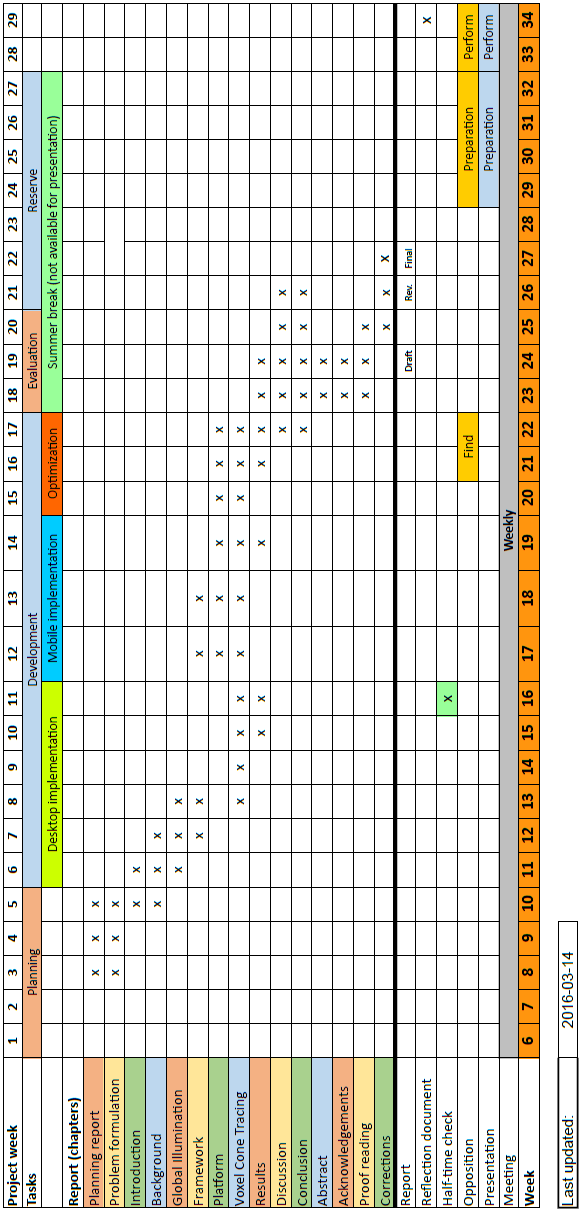
\includegraphics[scale=0.5]{images/timeplan.png}
    \label{fig:timeplan}
\end{figure}

\end{appendices}
\end{document}
